\chapter{Background and Related Work}
\label{ch:lit}

\section{Protocol Foundations}
\label{sec:background}

5G New Radio (NR) networks rely on precise uplink synchronization and orthogonal multiplexing to
maintain multi-user communication.

\subsection{Uplink Synchronization and Timing Advance}
Because multiple UEs share common uplink time-frequency resources, their transmissions must arrive at
the gNB aligned within a tight time window. Due to varying propagation distances, a UE must transmit
earlier than the nominal downlink frame boundary by an offset known as the Timing Advance (\TA{}):
\begin{equation}
  T_\mathrm{TA} = (N_\mathrm{TA} + N_{\mathrm{TA,offset}}) \cdot T_c ,
  \label{eq:ta_def}
\end{equation}
where $T_c = 1/(480\,000 \times 4096)\,\text{s} \approx 0.509$\,ns is the basic 5G time unit~\cite{3gpp38211}.
The gNB derives \TA{} by correlating received Random Access Channel (PRACH) preambles against expected
Zadoff-Chu sequences, reporting the delay of the largest correlation peak. In legacy operation, \TA{} is
dynamically updated via 6-bit closed-loop MAC CE adjustments to compensate for mobility.

\subsection{Cyclic Prefix and the Decodability Margin}
In 5G OFDM, each symbol is prepended with a Cyclic Prefix ($L_{\mathrm{CP}}$) to prevent inter-symbol
interference (ISI) from multipath delay spread. The cyclic prefix also absorbs small timing advance
errors. However, if the timing error exceeds $L_{\mathrm{CP}}$, adjacent symbols bleed into the FFT
window, destroying subcarrier orthogonality and causing abrupt decodability collapse.

\section{Lower-Layer Triggered Mobility (LTM)}
\label{sec:ltm}

LTM is standardized in TS~38.300~\cite{3gpp38300}, TS~38.321~\cite{3gpp38321}, and
TS~38.331~\cite{3gpp38331}, and has been characterized in the academic
literature~\cite{khodapanah2024ltm,atik2026evolution,lee2025enhanced}. Its operational workflow
comprises three phases (\cref{fig:ltmflow}):

\begin{figure}[htbp]
  \centering
  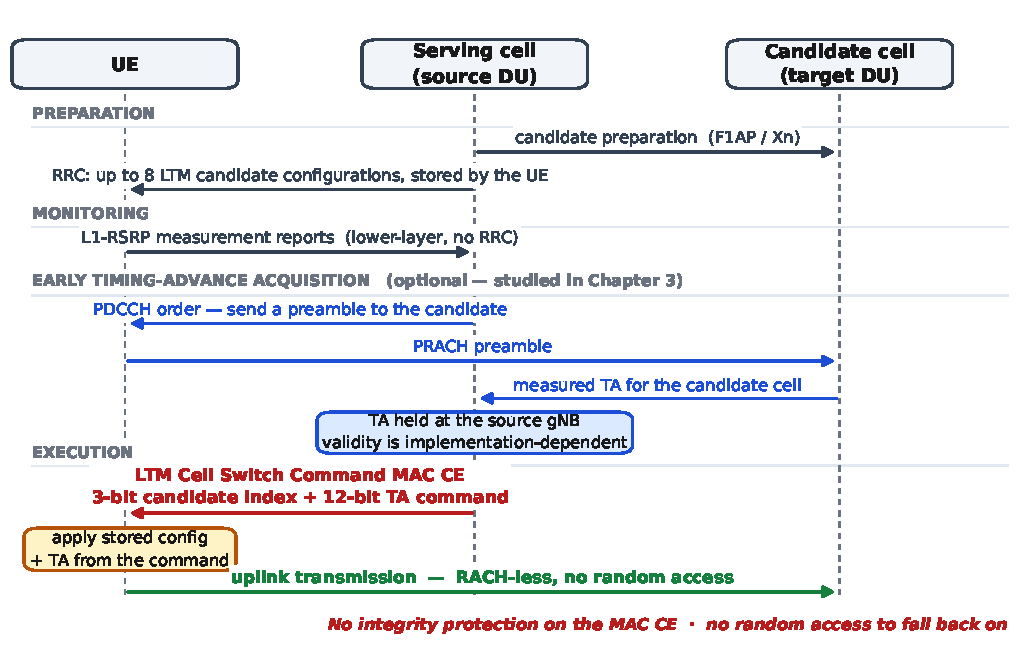
\includegraphics[width=\textwidth]{figures/ltm_flow.pdf}
  \caption{LTM procedure: preparation, monitoring, and execution. The optional early \TA{}
  acquisition phase pre-populates candidate \TA{} to enable RACH-less switching.}
  \label{fig:ltmflow}
\end{figure}

\begin{enumerate}\itemsep2pt
  \item \textbf{Preparation:} The serving gNB provisions up to eight candidate cell configurations
        to the UE via RRC. Configurations are pre-cached in UE memory, allowing subsequent switch
        commands to reference candidates via a compact 3-bit index.
  \item \textbf{Early Timing Advance Acquisition:} The network orders the UE to transmit a PRACH
        preamble to candidate cells prior to any handover~\cite{iqbal2024rachless}. The candidate DU
        measures the arrival delay,
        computes the \TA{}, and forwards it to the serving cell over F1AP. The basic \TA{} quantisation
        step is:
        \begin{equation}
          T_\mathrm{unit} = \frac{16 \cdot 64}{2^{\mu}}\, T_c ,
          \label{eq:taunit}
        \end{equation}
        evaluating to 520.8\,ns at $\mu=0$ (15\,kHz) and 260.4\,ns at $\mu=1$ (30\,kHz). One unit at
        $\mu=1$ corresponds to approximately 78\,m of one-way distance.
  \item \textbf{Execution (RACH-less):} When radio conditions warrant a switch, the serving cell transmits
        an LTM Cell Switch Command MAC CE containing the pre-calculated \TA{}. If a valid \TA{} is present,
        the UE skips the target cell RACH handshake and immediately commences transmission.
\end{enumerate}

\section{Related Work}

\paragraph{Handover and Low-Layer Attacks:}
Prior research demonstrates that cellular mobility procedures are vulnerable to unauthenticated inputs.
Shaik et al.~\cite{shaik2018rogue} demonstrated poisoning of self-organizing network (SON) handover
mechanisms. Bitsikas and Noubir~\cite{bitsikas2021donthandover} exposed vulnerabilities in unverified
RRC measurement reports. At layer~2, Erni et al.\ introduced AdaptOver~\cite{erni2022adaptover} and
5G-Overshadowing~\cite{erni20265gone}, showing that physical-layer signal overshadowing can reliably
inject unauthenticated MAC/RLC frames on commercial 5G networks. Luo et al.\ demonstrated SNI5GECT for
injection without a rogue base station~\cite{luo2025sni5gect}. Ludant et al.\ catalogued unprotected
low-layer control messages~\cite{ludant2025lowlayer} and demonstrated passive control sniffing via
5GSniffer~\cite{ludant2023sniffing}. Hamici-Aubert et al.~\cite{hamici2024overshadowing} forced RLC NACK
injections, inducing measurable transmission delays.

\paragraph{Scheduling Request Procedure Robustness:}
While low-layer scheduling and mobility procedures have been analyzed independently, no prior academic
study or 3GPP Change Request has investigated the interaction between the Scheduling Request retry
mechanism (TS~38.321 clause~5.4.4) and RACH-less LTM execution, searched via the 3GPP specification
change database and the academic literature cited in this section. \Cref{sec:m2gap} returns to this gap
with the decisive specification-level evidence that it is an omission rather than a deliberate design
choice.

\paragraph{Timing Advance Manipulation:}
\label{sec:lit-ta}
Kwao et al.~\cite{kwao2024random} demonstrated random access desynchronization attacks. Shanto, Karim,
and Bertino~\cite{shanto2026breaking} analyzed timing advance manipulation on commercial UEs, identifying
radio link failure (RLF) thresholds between 20 and 60 units. This figure is 3--10$\times$ larger than the
6--8 unit decodability boundary this report measures (\cref{sec:r1boundary}), but the two are not directly
comparable: Shanto et al.\ manipulate the \emph{serving} cell's actively closed-loop-tracked \TA{} and
measure \emph{RLF}, a downlink out-of-sync \emph{counter} that integrates over repeated measurement
intervals and is continuously nudged back toward correctness by the tracking loop between attacks; this
report instead measures the one-shot coded block-error rate of a single \emph{candidate}-cell uplink
transmission made with a \TA{} that was corrupted once, during early acquisition, and never
closed-loop-corrected before use. A UE tolerating a larger error before its serving-cell RLF counter
expires is accordingly not evidence that a freshly-applied, uncorrected candidate \TA{} would survive the
same error on its first transmission; reconciling the two thresholds on a common commercial receiver
remains open work, noted in \cref{sec:limits}.

\paragraph{MAC Control Element Security:}
Cao et al.~\cite{cao2025macce} surveyed MAC CE security broadly. Hätinen's 2026 study with
Ericsson~\cite{hatinen2026overshadowing} analyzed overshadowing across 69 MAC CEs. However, Hätinen's
analysis assumed that \TA{} corruption would be resolved by \texttt{timeAlignmentTimer} expiry and
subsequent RACH fallback. Crucially, that analysis pertained only to Conditional LTM (CLTM, clause
5.2), where a UE-side timer exists. Under plain LTM (clause 6.1.3.75), \TA{} is held by the network with
no UE-side timer and no fallback mechanism.

\paragraph{Handover Anomaly Detection:}
Dey and Patra~\cite{dey2025secure,dey2023handitover} proposed detecting handover DoS attacks in 5G-V2X
using machine learning classifiers trained on radio link failure and handover statistics.

\section{Research Gap}
\label{sec:gap}

Prior literature reveals two fundamental limitations:
\begin{enumerate}\itemsep2pt
  \item \textbf{Serving vs.\ Candidate Timing Advance:} Existing timing attacks target the serving cell,
        where closed-loop adjustments continuously correct drift, forcing an adversary to remain active.
        No prior work has examined candidate \TA{} values acquired in advance and stored asynchronously in
        network-side state without continuous closed-loop feedback.
  \item \textbf{Message Forgery vs.\ Architectural Logic:} Most low-layer security studies focus on
        exploiting the lack of MAC CE integrity protection via message forgery. Consequently, they do not
        investigate the protocol vulnerabilities created by LTM's speed-up architecture itself---specifically,
        how unauthenticated cached state interacts with disabled recovery procedures during RACH-less
        switching.
\end{enumerate}
This report bridges this gap by uncovering flaws in 3GPP specification logic that survive cryptographic
MAC CE integrity protection.
